\chapter{Introduction}
This work was done in collaboration with Maya Heat Transfer Technologies, a company developing its own flow solver named NX Flow, part of the Siemens PLM portfolio. The aim of this thesis is the implementation and validation of the Spalart-Allmaras turbulence model in NX Flow as well as the in-house academic code at McGill's Computational Aerodynamics Group, named syn3D.


\section{Computational fluid dynamics}
Computational fluid dynamics (CFD) is a branch of fluid mechanics that uses numerical analysis to solve problems that involve fluid flows. The fundamental basis to all CFD problems is the Navier-Stokes equations, a set of mathematical equations governing the dynamics of any fluid flow. Surprisingly, numerical methods for CFD were first developed in the 1910's by Lewis Fry Richardson even prior to the first computers and were carried out by hand. Then, a team at the Los Alamos National Lab in 1957 developed the first functional CFD computer simulation model. Due to a lack of computational resources, only a simplified set of equations could be solved.

As computational resources became more abundant and the processor speed and available memory increased at a rapid rate, the full Navier-Stokes could finally be solved.
%
\section{Turbulence modelling}
%
In theory, the Navier-Stokes equations can be solved numerically, provided initial and boundary conditions. This is what is called Direct Numerical Simulation (DNS).  DNS for turbulent flows requires that all turbulent effects, which occur at very small temporal and spatial scales, be resolved. This is further discussed in~\Cref{sec:random}. Common solutions to this problem are given in~\Cref{sec:turbsolution}, namely large eddy simulation and the Reynolds-averaged Navier-Stokes (RANS) or Favre-averaged Navier-Stokes (FANS) equations. An introduction to the latter is given in~\Cref{sec:introrans}. The law of the wall, an important concept in turbulence modelling, is given~\Cref{sec:lawofthewall}. Finally, an overview of the Spalart-Allmaras model~\cite{spalart1994one}, which is the model to be implemented and validated, is given in~\Cref{sec:introsa}.
%
\subsection{Random nature of turbulence}
\label{sec:random}
%
The Reynolds number $\Rey$ is a dimensionless quantity commonly used to characterize fluid flows and is mathematically expressed as:
\begin{equation*}
    \Rey = \frac{\rho U l}{\mu},
\end{equation*}
where $l$ is a characteristic length and $U$ the velocity. The Reynolds number is a measure of the ratio of inertial forces to viscous forces. At low Reynolds numbers, fluid particles may follow relatively straight lines and minimal mixing occurs. For instance, a flow composed of a heterogeneous mixture may remain heterogeneous. This flow regime is referred to as laminar flow.

On the other hand, flow at high Reynolds numbers is rather chaotic and random. Fluid particles no longer follow straight lines and mixing is significantly increased. A heterogeneous mixture will quickly become homogeneous if it can. Flow properties such as velocity vary randomly in time and space, even if boundary conditions are constant. This regime is called turbulent flow. It also happens that many flows in engineering are turbulent~\cite{versteeg2007introduction}, as are all cases mentioned in the present work.

Turbulent flows are easily identifiable by the presence of vortices, or eddies, in the flow. Such a phenomenon was observed and documented as far back as the 15th century, by none other than Leonardo Da Vinci. \Cref{fig:vinci} depicts his studies of vortices in turbulent fluid motion. The lower drawing in this figure shows the formation of eddies of various sizes that is typical of turbulent flows. These eddies typically manifest themselves in the vicinity of velocity gradients, such as in free shear flows or near solid boundaries. The physical reason for which DNS is so costly is that it must resolve the production and decay of eddies in order to accurately simulate the flow.

The number of mesh points $N$ required to resolve turbulent effects can be related to the Reynolds number by~\cite{wilcox1998turbulence}:
\begin{equation*}
    N = \Rey^{2.25}.
\end{equation*}
Hence, memory storage requirements and CPU time grow significantly with the Reynolds number. In addition, the time step size must be reduced such that a fluid particle moves only a fraction of the mesh spacing. Thus, computational costs involved in DNS are too large for even simple problems in the turbulent regime. For instance, resolving the flow field over an airfoil at $\Rey$ = 5 million, a typical flight Reynolds number, would require $10^{15}$ mesh points. For comparison, simulations that are considered ``large'' today are typically comprised of $10^{8}$ mesh points, and those can only be solved on massively parallel supercomputers.

\begin{figure}
    \centering
    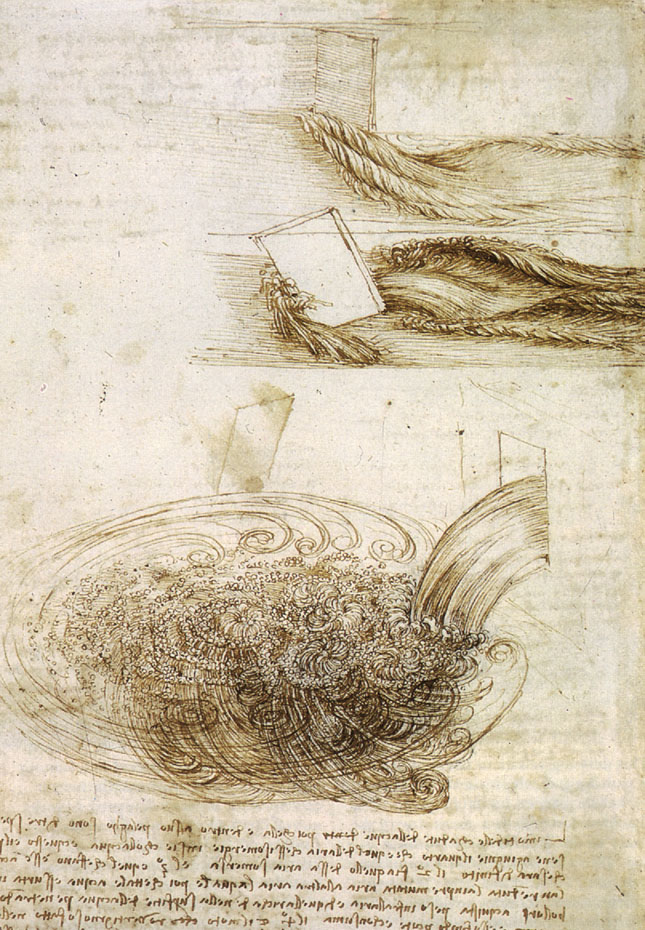
\includegraphics[width=0.3\textwidth]{figs/vinci}
    \caption{Studies of vortices in turbulent fluid motion by Leonardo da Vinci~\cite{wiki:vinci}.}
    \label{fig:vinci}
\end{figure}

Readers are referred to~\cite{pope2001turbulent,wilcox1998turbulence} for a more thorough discussion of turbulence.

\subsection{Alternatives to DNS}
\label{sec:turbsolution}
As discussed in the previous section, it is extremely costly to numerically resolve turbulent effects, which makes it impossible to perform simulations on real-life engineering cases using DNS. At the expense of accuracy, it is possible to instead model these effects. A common approach is to employ an averaging technique called Reynolds averaging and solve the Reynolds-averaged Navier-Stokes equations, which yield a solution for the mean flow. This approach is further detailed in~\Cref{sec:turb}.

Another approach, large eddy simulation (LES), which is more costly but typically yields a more accurate solution than RANS, resolves most of the turbulence effects while modelling the smaller scales through low-pass filtering functions. Such a filtering effectively removes small-scale information from the numerical solution, allowing a coarser mesh than DNS to be used.
%
\subsection{Reynolds Averaging}
\label{sec:introrans}
%
For most engineering purposes it is unnecessary to resolve every detail of the turbulent fluctuations. In other words, merely solving for the so-called mean flow would be satisfactory. This would require a set of equations that is only concerned with the mean quantities of the flow. The most common, and probably simplest, way to obtain the mean flow equations is to write all conserved quantities appearing in the conservation equations as a sum of a fluctuating component and a mean component. Taking for instance an instantaneous conserved quantity $\phi$, one can write:
\begin{align*}
    \phi &= \ravg{\phi} + \phi'\\
    \ravg{\phi} &= \frac{1}{\text{T}} \int_{\text{T}}\phi(t)
        ~\text{d}t,
\end{align*}
where $\ravg{\phi}$ is the mean component, $\phi'$ is the fluctuating component, and $\text{T}$ is a time interval longer than the characteristic time scale of the turbulence. The mean component is then a time-averaged value, which is only relevant in statistically stationary (steady) flows. This work is only concerned with such flows. This technique is called a Reynolds decomposition.

To allow for compressibility effects, a mass weighted average must also be introduced. The Favre decomposition is defined as:
\begin{align*}
    \phi &= \favg{\phi} + \phi'' \\
    \favg{\phi} &= \frac{\overline{\rho\phi}}{\overline{\rho}}.
\end{align*}
It is important to note that $\ravg{\phi'} = 0$ but $\ravg{\phi''} \ne 0$.

In order to obtain a set of mean governing equations, a Reynolds decomposition for pressure and density and a Favre decomposition for velocity, internal energy and temperature is taken and substituted into the original (instantaneous) Navier-Stokes equations. Next, a time average of the resulting equations is taken. This leads to the Favre-averaged Navier-Stokes equations. As shown in~\Cref{sec:fans}, this introduces six new unknowns, which are the components of the symmetric Reynolds stress tensor. Since no additional equations are introduced, the system of equations is under-determined. This is the closure problem of turbulence.

A common solution to this problem, which is further detailed in~\Cref{sec:bouss}, is to approximate the Reynolds stress tensor as a function of density, velocity and a new quantity $\mu_T$ called the \emph{turbulent eddy viscosity}. This solution is referred to as the Boussinesq approximation.
% This new variable is solved for through a \emph{turbulence model}, which provides an additional equation for $\mu_T$; the Spalart-Allmaras model is one example of a turbulence model.
%
\subsection{Law of the wall}
\label{sec:lawofthewall}
%
The total shear stress is the sum of viscous and Reynolds stresses. The Reynolds stresses being null at a wall, since $\vec{u} = 0$, the total shear stress at the wall $\tau_w$ is due entirely to the viscous contribution. It was found through experimentation and simulation that the Reynolds stresses tend to dominate as one moves away from the wall~\cite{pope2001turbulent}. In fact, the relative importance of both sources of stress can be determined through a non-dimensional wall distance $y^+$ defined by:
\begin{equation*}
    y^+ = \frac{u_\tau d}{\nu},
\end{equation*}
where $d$ is the distance to the nearest wall and $u_\tau$ is the friction velocity defined as:
\begin{equation*}
    u_\tau = \sqrt{\frac{\tau_w}\rho}.
\end{equation*}
It is possible to identify the following layers in the near-wall flow based on the $y^+$ value:
\begin{description}
    \item[Viscous sublayer] ($y^+ < 5$): Viscous stresses dominate
    \item[Buffer layer] ($5 < y^+ < 30$): Neither stress dominates
    \item[Log-law layer] ($y^+ > 30$): Turbulent stresses dominate
\end{description}
Another quantity of interest is the non-dimensional velocity $u^+ = U/u_\tau$ where $U$ is the velocity parallel to the wall, which can be related to $y^+$ through a function $f_w(y^+)$. For fully turbulent flows, the function $f_w$ has been found to be universal and to vary depending on the layer as follows:
\begin{description}
    \item[Viscous sublayer]: $u^+ = y^+$
    \item[Log-law layer]: $u^+ = \frac{1}{\kappa} \ln y^+ + C^+$
\end{description}
where $\kappa \approx 0.41 $ is the Von Kármán constant and $C^+\approx5.0$ for a smooth wall~\cite{pope2001turbulent}. There is no clear relationship between $u^+$ and $y^+$ in the buffer layer, as the contributions to the shear stress are mixed.

In CFD packages that solve the averaged equations, it is recommended to have at least a few points within the viscous sublayer in order to resolve the flow correctly. Thus, in practice, the computation of $y^+$ is useful in determining whether the mesh requires refinement.
%
%
\subsection{Spalart-Allmaras model}
\label{sec:introsa}
%
%
Solving the RANS equations requires evaluation of the eddy viscosity, the quantity that models the effects of turbulence. This quantity is solved for through a turbulence model. One such turbulence model is called the Spalart-Allmaras (SA) model~\cite{spalart1994one}, and is the focus of this work. This particular model was designed for aerospace applications and has been shown to give good results for boundary layers subject to adverse pressure gradients~\cite{spalart1994one}. The model has already been implemented in various CFD codes, both cell-centered~\cite{bardina1997turbulence,seror2005implementation,trompoukis2011cuda,saxena2002implementation} and vertex-centered~\cite{anderson1994implicit,gerhold1997calculation,wang2010comparison}. It also involves solving only one additional transport equation, as opposed to other turbulence models such as the $k-\epsilon$ and $k-\omega$ models which require solving two equations. Thus, the Spalart-Allmaras model offers a good trade-off between computational cost and solution accuracy and is well suited for the cases discussed in this work. Another reason for the choice of this model is that a customer of NX Flow requested it. Details and variants of the SA model are given in~\Cref{sec:sa}.

The SA equation depends on the distance to the nearest wall, which can be calculated in various ways, as shown in~\Cref{sec:walldist}. While the Navier-Stokes equations do not depend on such a quantity, it is important to accurately compute this distance in order to correctly predict the behavior of turbulent flows using the Spalart-Allmaras model. In fact, this value is required by most turbulence models, including the two-equation models mentioned above.

\section{Thesis overview}
The governing equations and an introduction to turbulence modelling are presented in~\Cref{chap:governing}. Numerical methods and their implementation in both solvers are given in~\Cref{chap:num}, which shows the differences in implementation between both codes.

Results are presented in~\Cref{chap:results} and compared against either experimental data or other established CFD codes. The goal is to demonstrate that the implementation in both codes is correct and also to highlight the differences in results that arise due to the different implementations. Special importance is given to the boundary conditions, since they can significantly affect the solution. Specifically, this work aims to determine if the implemented boundary conditions are suitable for external flows and to assess their impact on grid sensitivity.

For some cases, a grid study is performed, in which the same problem is solved on successively finer computational grids. Such a study aims to determine whether grid is sufficiently refined such that the solution lies in the asymptotic range of convergence~\cite{roache1986editorial}, which is obtained when the grid size no longer significantly affects the result. This type of study will be used to assess the sensitivity of the solution on grid density for both codes. The effects of grid size on the convergence of the residual will also be investigated.

Problems to be solved involve both compressible and incompressible cases; the accuracy of each solver for these types of flow will be discussed.

